\documentclass[oneside,senior,etd]{BYUPhysForDegree}

\usepackage[utf8]{inputenc}
\usepackage{rotating} 

\usepackage[russian]{babel}
\usepackage{amsfonts} % Пакеты для математических символов и теорем
\usepackage{amstext}
\usepackage{amssymb}
\usepackage{amsthm}
\usepackage{graphicx} % Пакеты для вставки графики
\usepackage{subfig}
\usepackage{color}
\usepackage[unicode]{hyperref}
\usepackage[nottoc]{tocbibind} % Для того, чтобы список литературы отображался в оглавлении
\usepackage{algorithmic} % Для записи алгоритмов в псевдокоде
\usepackage{algorithm}
\usepackage{verbatim} % Для вставок заранее подготовленного текста в режиме as-is
\usepackage{listings}

\usepackage{commath}
\newcommand\Tau{\mathcal{T}}
\newcommand{\R}{\mathbb{R}}
\usepackage{color}
\usepackage[colorinlistoftodos, prependcaption]{todonotes}
\usepackage{multirow}
\newcommand*{\MyIndent}{\hspace*{0.2cm}}%

\Chair{Кафедра автоматизации систем вычислительных комплексов}
\Lab{~}
\Year{2022}
    \Month{Август}
    \City{Москва}
    \AuthorText{Автор}
    \Author{Арефьев Вениамин Андреевич}
    \AuthorEng{}
    \AcadGroup{321}
    \TitleTop{Разработка методов нагрузочного тестирования}
    %\TitleMiddle{}
    \TitleBottom{распределённой файловой системы lustre} % leave empty if you don't need it
    \TitleTopEng{}
    \TitleBottomEng{} % leave empty if you don't need it  
    \docname{Курсовая работа}
    %\docname{Выпускная квалификационная работа}
    %\docname{Магистерская диссертация}
    \Advisor{Сальников Алексей Николаевич}
    \AdvisorDegree{в.н.с., к.ф.-м.н.}
    %\Consultant{}
    %\ConsultantDegree{}
  
\Abstract{
В вычислительном  кластере всегда используется какая-либо параллельная файловая система, и у неё есть
некоторые теоретические характеристики. Часто возникает потребность измерить реальную производительность
файловой системы для каждого узла и кластера в целом, а так же проверить стабильность работы системы при
нагрузке, в том числе на специальном стенде для проектирующегося кластера. 
Часто в кластерах используется распределённая по вычислительной системе файловая система lustre. Для
параллельного запуска программы на всех узлах используется библиотека MPI. В работе для создания
нагрузки на сеть использовались операции ввода-вывода в файлы из MPI-IO: часть MPI. Пользователю системы
тестирования предоставляется возможность получить список производительности операций чтения-записи на
определённом наборе тестов. Результаты тестирования позволяют предпринять соответствующие меры для
поднятия производительности вычислительной системы, построенной поверх оборудования кластера, при
необходимости. Данная программа была протестирована на тестовых стендах и реальном суперкомпьютере
МВС-10П.

Ключевые слова: Тестирование параллельной файловой системы, файловая система lustre, высокопроизводительные
вычисления(HPC), MPI, MPI-IO, тестирование ввода-вывода(IO testing), суперкомпьютеры, организация файлового 
хранилища (storage infrastructure)
}
%\AbstractEng{Abstract}
\AbstractEng{}


%%%% DON'T change this. It is here because .sty does not support cyrillic cp properly %%%%
\University{Московский государственный университет имени М.В.Ломоносова}
\Faculty{Факультет вычислительной математики и кибернетики}
\GrText{гр.}
\AdvisorText{Научный руководитель}
%\ConsultantText{Научный консультант}
\AbstractText{Аннотация}

\begin{document}
\fixmargins
\makepreliminarypages

\oneandhalfspace

\tableofcontents

\section{Введение}
\label{sec:Chapter0} \index{Chapter0}


В настоящее время суперкомпьютеры, в частности, вычислительные кластеры являются достаточно мощными
инструментами для решения огромного спектра задач ~\cite{Zheng2018InteractiveCO}
~\cite{hoefler2014overview}~\cite{bezrukov2018machine}.
Они применяются в вычислительных целях в том случае,
когда задачу можно разделить на несколько подзадач, каждая из которых может выполняться на отдельном узле.
Большое количество ученых используют их для проведения своих расчётов в научных работах, математическом
моделировании и обработке больших объемов данных.

Данные задачи требуют мощных вычислительных ресурсов,
поэтому суперкомпьютеры стали прекрасным инструментом, который удовлетворяет таким высоким требованиям.
Например:
\begin{description}
    \item[$\bullet$] Различные нефтегазовые компании используют суперкомпьютеры для обработки
    сейсмических данных и нахождений новых месторождений природных ископаемых. Собранные сейсмические морские данные могут составлять терабайты информации и требовать более сотни часов на обработку специальными алгоритмами на машине Factor 2000 (~10 терафлопс в секунду). ~\cite{Meuer2013SupercomputersP}
    \item[$\bullet$] Прогноз погоды занимает около 25 часов при средней производительности в 115
    терафлопс в секунду.~\cite{Open_Forecast_HPC_Model_M04} 
    \item[$\bullet$] Численное моделирование в аэродинамике летательных аппаратов. Вычислительная
    гидродинамика требует производительности хотя бы 50 терафлопс в секунду, чтобы завершаться за
    приемлемое время (порядка нескольких дней).  ~\cite{Meuer2013SupercomputersP}
    \item[$\bullet$] Моделирование населения Галактики во Вселенных Темной энергии: Проект
    Millennium-XXL. Данный проект работал на суперкомпьюере JUROPA с производительностью 275 терафлопс в
    секунду и оперативной памятью 30 терабайт. При этом сгенерировав 100 терабайт данных.  
    ~\cite{Open_Forecast_HPC_Model_M04} 
\end{description}



У каждого суперкомпьютера есть своя файловая система. Файловая система --- это порядок, определяющий
способ организации, хранения и именования данных на носителях информации. Файловая система определяет
формат содержимого и способ физического хранения информации, которую принято группировать в виде файлов.
Обычно используются распределённые файловые системы --- это такие системы, в которых доступ к физически
распределённым данным осуществляется посредством тех же интерфейсов, что и к локальным данным.


Главные преимущества распределенных файловых систем:

Сетевая прозрачность - обеспечение тех же самых возможностей доступа к файлам, распределенным по сети
ЭВМ, которые обеспечиваются в системах разделения времени на централизованных ЭВМ.
~\cite{distributed_operating_systems_course}

Высокая доступность - ошибки систем или осуществление операций копирования и сопровождения не должны
приводить к недоступности файлов.~\cite{distributed_operating_systems_course}


Далее будем рассматривать только распределённую файловую систему lustre, потому что она является
бесплатно распространяемой файловой системой с открытым исходным кодом и часто встречается среди суперкомпьютеров 
из рейтинга top500~\cite{top500}.

Для одновременного запуска программы на всех узлах кластера, синхронизации во время запуска тестов и
последующего сбора результатов тестирования используется Message Passing Interface (MPI) --- программный 
интерфейс (API) для передачи информации, который позволяет обмениваться сообщениями между процессами,
выполняющими одну задачу и расположенными на разных физических машинах. 
MPI является наиболее распространённым стандартом интерфейса обмена данными
в параллельном программировании, существуют его реализации для большого числа компьютерных платформ.
Он используется при разработке программ для кластеров и суперкомпьютеров. Основным средством коммуникации
между процессами в MPI является передача сообщений друг другу.

Когда речь заходит о высокопроизводительных вычислениях сразу вспоминаются самые низкоуровневые
языки программирования, такие как Assembler, С, С++. Для наибольшей универсальности конечной программы
был выбрал язык C, и стандарт языка версии C99.

Поскольку настройкой вычислительных кластеров всегда занимается человек, то последний может совершать
ошибки, вследствие чего в некоторых случаях может наблюдаться резкое падение производительности каких-либо
частей вычислительной системы. В частности, при неправильной конфигурации файловой системы может
происходить уменьшение как средней, так и максимальной скорости чтения-записи файлов. Но эту проблему
можно отследить, если провести нагрузное тестирование файловой системы и выявить при каких условиях
возникают данные проблемы. Но чтобы снегенировать правильную нагрузку, нужно знать какие части системы
могут с ней не справиться, поэтому нужно изучить устройство конкретной файловой системы.

 % Введение
\section{Постановка задачи}
\label{sec:Chapter1} \index{Chapter1}


Существует вычислительный кластер с возможностью запуска MPI программ. На нём настроена и примонтирована
на каждом вычислительном узле файловая система lustre.

Для того, чтобы понять в каких местах происходит падение производительности и выяснить, происходит ли оно, необходимо провести нагрузочное тестирование, ориентированное на компоненты файловой системы. Если скорость чтения-записи будет падать на каких-либо тестах, то можно обозначить проблемные участки. 

А для того, чтобы провести нагрузочное тестирование, необходимо определить набор тестов, которые
будут использоваться при работе программы. Реализация программы должна удовлетворять следующим требованиям:

\begin{description}
    \item[$\bullet$] Программа должна в автоматическом режиме собирать информацию с узлов кластера,
    анализировать её и выводить конечному пользователю.
    
    \item[$\bullet$] После работы программы не должно оставаться никаких дополнительных файлов, которые
    создавались в процессе тестирования.
    
    \item[$\bullet$] Результаты работы программы не должны разительно отличаться между различными
    запусками (отличие результатов более чем в 2 раза считается достаточным, чтобы можно было говорить об
    ухудшении производительности).

    \item[$\bullet$] Тестирующая программа должна иметь возможность адаптироваться к количеству узлов, на которых будет запущена.
\end{description}
 % Постановка задачи
\section{Обзор существующих решений}
\label{sec:Chapter2} \index{Chapter2}

Многие существующие решения имеют гораздо больший функционал и большое количество зависимостей,
что сильно ограничивает область их применения. Также имеется достаточно большой спект коммерческих
решений с закрытым исходным кодом. Далее будут разобраны несколько утилит с открытым исходным кодом.
После их анализа будет сформирован подход к написанию тестов на каждом узле. А после будет добавлен
параллельный запуск этих программ на всех узлах одновременно.

\subsection{Тесты из официального дистрибутива Lustre}
На официальной сайте распределённой файловой системы Lustre можно найти несколько статей о
тестировании данной файловой системы~\cite{lustre_tests}. В основном там представлены тесты,
направленные на тестирование функциональности файловой системы и различных её компонентов, например: 
\begin{description}
    \item[$\bullet$] \textbf{conf-sanity}.
    
    Набор модульных тестов, которые проверяют инструменты настройки и запускают Lustre с несколькими
    различными настройками для обеспечения правильной работы в необычных конфигурациях системы.
    \item[$\bullet$] \textbf{insanity}
    
    Набор тестов, которые проверяют множественные одновременные условия отказа в обслуживании (выключение) компонентов файловой системы lustre и последующее автоматическое возобновление работоспособности.
    \item[$\bullet$] \textbf{sanity}
    
    Регрессионное тестирование - собирательное название для всех видов тестирования программного обеспечения, направленных на обнаружение ошибок в уже протестированных участках исходного кода. 
    
    Набор регрессионных тестов, которые проверяют работу в штатных условиях эксплуатации, когда всем систему функционируют без сбоев. Они тестируют большое количество необычных операций, которые ранее вызывали проблемы с функциональностью или корректностью данных в Lustre.
    
    \item[$\bullet$] \textbf{sanity-dom}
    
    Проверка корректности данных на серверах метаданных.
    \item[$\bullet$] \textbf{sanity-flr}
    
    Проверка корректности дублирования на уровне файлов.
    \item[$\bullet$] \textbf{sanity-lnet}
    
    Тест на корректность для lnet
    \item[$\bullet$] \textbf{sanity-quota}
    
    Набор тестов, которые проверяют корректронсть работы квот файловой системы. То есть запрет пользователям использовать ресурсов больше, чем им выделено.
    \item[$\bullet$] \textbf{sanity-sec}
    
    Проверяет функции идентификации Lustre, включая сопоставление \textbf{UID/GID}
\end{description}

Эти тесты проверяют множество различных составных частей данной системы, эмулируя
различные ситуации, например, отказ некоторых компонентов или создание множества
параллельных запросов к файловой системе.

Данные тесты стоит запускать, если нагрузочное тестирование показывает очень плохие результаты относительно теоритически рассчитаной пропускной способности.

Также есть и различные тесты производительности: ~ \cite{lustre_tests}
\begin{description}
    \item[$\bullet$] lnet-selftest
    
    Это модуль ядра, который работает через внутренюю сеть файловой системы LNET и сетевые драйверы Lustre (LNDs). Он предназначен для проверки возможности подключения сети Lustre, выполнения
    регрессионных тестов и тестирования производительности сети Lustre.
    \item[$\bullet$] obdfilter-survey
    
    Этот скрипт исследования выполняет последовательный ввод-вывод с различным
    количеством потоков и объектов (файлов).
    \item[$\bullet$] sgpdd-survey
    
    Это исследование может быть использовано для охарактеризования производительности переферийного
    устройства. Он имитирует сервер хранения данных, обслуживающий несколько распределённых между
    логическими томами файлов. Данные, собранные им, могут помочь определить ожидания относительно
    производительности при использовании его в качестве сервера хранения данных Lustre.
    \item[$\bullet$] bonnie++
    
    Bonnie++ тест применяется для создания, чтения и удаления множества небольших файлов, и изменения их метаданных. В резулатате своей работы он даёт пользователю производительность его файловой системы в виде скорости чтения-записи.
    \item[$\bullet$] dbench
    
    Тест Dbench используется для моделирования использования файловой системы N клиентами. Полученные в результате выполнения программы данные могут быть интерпретированы как максимальная пропускная способность операций ввода-вывода данной файловой системы.

    \item[$\bullet$] fsx
    
    Тестировщик файловой системы был разработан вне Lustre и предназначен для
    стресс-тестирования необычных операций ввода-вывода и файловых операций.
    Он проверяет целостность данных после каждого шага. 
    \item[$\bullet$] iozone
    
    Тест Iozone применяется для генерации и измерения различных файловых операций.
    
\end{description}

Данные решения производят хорошее нагрузочное тестирование как отдельных элементов файловой системы,
так и всей системы в целом. В частности все они предоставляют информацию о пиковой и средней скорости чтений-записи файлов на диск.

\subsection{Flexible Input/Output}

В официальном репозитории можно найти много полезной информации.\cite{fio}

Изначально FIO был написан, чтобы избавиться от необходимости писать специальные
программы для тестирования, когда человек хочет протестировать определенную рабочую
нагрузку либо по соображениям производительности, либо для поиска/воспроизведения ошибки.
Процесс написания такого тестового приложения может быть утомительным, особенно если
приходится делать это часто. Следовательно, нужен был инструмент, который мог бы имитировать
заданную загруженность ввода-вывода и не заставлял бы прибегать к самостоятельному написанию
теста снова и снова.

Однако, тестовую рабочую нагрузку определить сложно. Может быть задействовано любое количество
процессов или потоков, и каждый из них может использовать свой собственный способ генерации
ввода-вывода. Может быть несколько потоков, будут выполнять запись в разные места одного файла одновременно или выполнять чтение с использованием асинхронного ввода-вывода. FIO должен
быть достаточно гибким, чтобы имитировать оба этих случая и многое другое.

FIO порождает несколько потоков или процессов, выполняющих определенный тип действий ввода-вывода,
как указано пользователем. FIO принимает ряд глобальных параметров, каждый из которых наследуется
потоком, если не указано иное. Типичное использование FIO заключается в записи используемого в
работе файла, соответствующего нагрузке ввода-вывода, который требуется имитировать.\newline\newline\newline

Все эти решения очень хорошо тестируют производительность для одного узла файловой системы,
но ими нельзя протестировать два или более узлов одновременно, что является неприемлимым для
тестирования производительности файловой системы вычислительного кластера. Именно поэтому на 
их основе нужно сформировать методику тестирования файловой системы для одного узла и впоследствии
её распараллелить. Так же из вывода программы должно быть понятно, на какие элементы системы следует
обратить внимание при поиске проблемного места.

 % Обзор существующих решений
\section{Исследование и построение решения задачи}
\label{sec:Chapter3} \index{Chapter3}

Рассмотрим все компоненты люстры и обратим внимание на те места, где может образоваться бутылочное горлышко.

\subsection{Устройство параллельной файловой системы Lustre}

\begin{figure}[h]
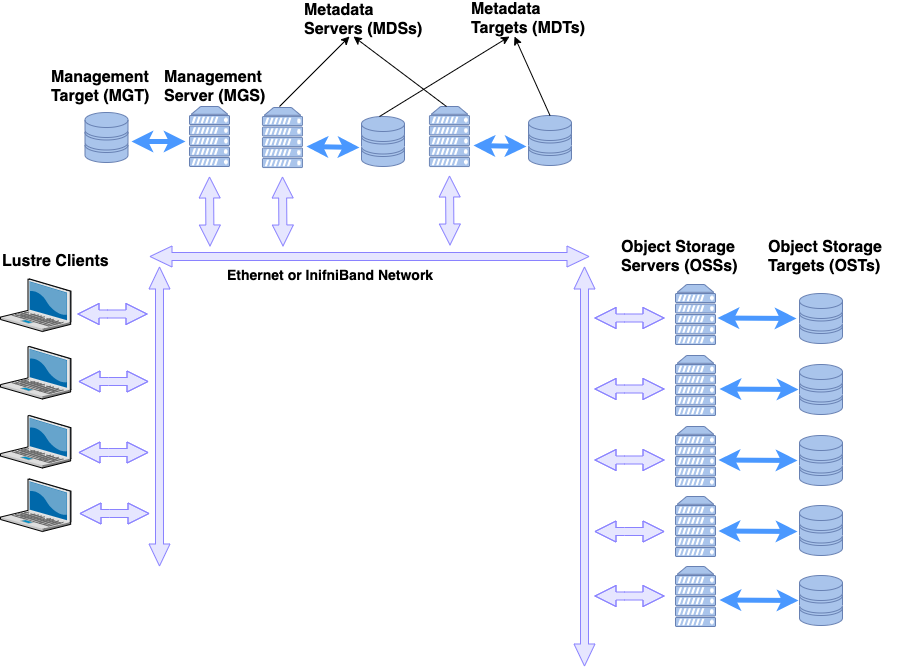
\includegraphics[height=12.5cm,keepaspectratio]{./lustre_components.png}\\[0.1cm]
\caption{Основные компоненты файловой системы Lustre}
\label{lustre_components}
\end{figure}

Существуют сервера управления и подконтрольные им сервера, которые называются соответственно Server и Target. 


MDS(Metadata Server) --- эти сервера отвечают за все операции над пространствами имён всей файловой системы Lustre. Вся информация
об иерархии директорий и метаданных файлов хранится на Target серверах, а MDS предоставляет логический интерфейс
для этих данных. В файловой системе всегда есть как минимум один MDS и соответствующий ему MDT, серверов второго 
типа может быть добавлено больше, чтобы удовлетворить запросы конкретной среды. Сервера метаданных управляют
распределением объектов хранения между серверами OSS для содержимого при создании файлов, а также управляют 
открытием и закрытием файлов, их удалением и переименованием и другими операциями над пространствами имён.

А на серверах MDT (Metadata Target) фактически хранится вся метаинформация пространства имён, такая как имена файлов, директорий,
права доступа, расположение файлов и индексы данных для эффективного доступа к хранимым в файловой системе данным.
Возможность иметь несколько MDT в одной файловой системе позволяет поддеревьям каталогов храниться на вторичном
MDT, что очень полезно для изоляции рабочих нагрузок, которые особенно интенсивно потребляют метаданные на
выделенном оборудовании (например, отдельный сервер MDT может быть выделен для определённого набора проектов).
Большие каталоги могут быть распределены по нескольким MDT, обеспечивая масштабируемость для приложений,
которые генерируют очень большое количество файлов в плоской иерархии директорий (множество файлов хранится в одной директории, а не разделяется между несколькими).

OSS(Object Storage Server) обеспечивает массовое хранение содержимого файлов в файловой системе Lustre. Один или несколько серверов хранения
данных OSS хранят данные файлов на одном или нескольких OST (Object Storage Target), в одной файловой системе Lustre могут быть тысячи 
серверов OSS. Обычно один OSS обслуживает от двух до восьми серверов OST (хотя возможно намного больше).
Ёмкость файловой системы Lustre это сумма всех ёмкостей, предоставляемых серверами хранения данных OSS через сервера OST.
OSS обычно конфигурируются парами, причём каждая пара подключается к общему внешнему хранилищу, которая
хранит сервера OST. Данный пример можно увидеть на рисунке~\ref{lustre_components}
Сервера OST доступны через два сервера в конфигурации активной и пассивной отказоустойчивости
для поддержания высокой доступности даже в случае каких-либо сбоев. OST монтируются только на одном сервере
одновременно и обычно равномерно распределены между всеми OSS для балансирования производительности и
максимизации пропускной способности.


MGS(Management Server) --- сервер управления, он хранит всю информацию о конфигурациях для всех файловых систем Lustre в кластере и
предоставляет эту информацию другим хостам Lustre. Сервера и клиенты подключаются именно к MGS при запуске,
чтобы получить конфигурации файловой системы. Уведомления обо всех изменениях в конфигурациях файловой системы,
включая перезагрузки серверов, распространяются именно MGS.
Постоянная информация для всех узлов кластера запоминается и записывается на устройства хранения, называемые MGT (Management Target).
MGS может быть совмещён с сервером MDS в конфигурации с очень высокой доступностью, при этом каждый сервер
подключен к общему хранилищу. Несколько файловых систем Lustre могут управляться только одним MGS.


Клиенты --- приложения получают доступ к данным файловой системы и используют их, взаимодействуя с клиентами Lustre.
Клиент Lustre представлен в виде точки монтирования файловой системы на хосте и предоставляет приложениям единое
пространство имен для всех файлов и данных в файловой системе, используя стандартную семантику POSIX. Файловая
система Lustre, установленная в клиентской операционной системе, очень похожа на любую другую файловую систему
POSIX; каждый экземпляр Lustre представлен как отдельная точка монтирования в операционной системе клиента, и
каждый клиент может монтировать несколько разных экземпляров файловой системы Lustre одновременно.

Рисунок ~\ref{lustre_components} показывает упрощенную версию компонентов файловой системы Lustre в базовом кластере. На этом рисунке сервер MGS физически отделён от серверов MDS, но для небольших файловых систем MGS и MDS могут быть объединены в один сервер, а MGT может сосуществовать на том же блочном устройстве, что и основной MDT.

\subsection{Возможные места высокой нагрузки}

\begin{description}
    \item[$\bullet$] Сервера метаданных при большом количестве создания, удаления и изменения данных о файле
    \item[$\bullet$] Сервера хранения данных при интенсивных операциях чтения-записи
    \item[$\bullet$] Сеть передачи данных файловой системы
\end{description}

Будем считать, что запас производительности сети пропускного канала настолько большой, что ошибок не будет
случаться, то есть, пакет всегда дойдёт до адресата. Поэтому будем тестировать другие составляющие системы.
 % Исследование и построение решения задачи
\section{Описание практической части}
\label{sec:Chapter4} \index{Chapter4}

\subsection{Описание программной реализации}

Для написания данной программы рассматривались 3 языка программирования: Ассемблер, С и С++. Ассемблер
практически сразу был исключен из рассмотрения в виду его крайне большой зависимости от конечной платформы.
Но следующий выбор уже не был таким очевидным, ведь С и С++ очень похожи. В конечном счёте выбор
был сделан в пользу C, т.к. он даёт больше контроля программисту над тем, что делает программа, и
над памятью, которая выделяется и используется в программе.

А в качестве инструмента параллельного запуска на всех узлах был выбран MPI стандарта 3.1 как
самый младший из наиболее часто установленных стандартов.

При запуске программа ничего не читает со стандартного ввода, а только анализирует аргументы командной
строки. Первый аргумент является обязательным и представляет из себя размер файла, который будет
записывать на диск. Второй и последующие аргументы является опциональными и должны представлять из себя
цифры от 1 до 6, таким образом указываются тесты, которые будут производиться. Если будет указан только
первый параметр, то будут запущены все тесты.

После работы главный процесс собирает все данные и выводит на стандартный вывод 12 чисел с плавающей
точкой, разделенные пробелом. Первые шесть цифр - это скорость записи файлов на диск (байт в секунду), а
последние 6 - это скорость чтения файлов с диска (байт в секунду).

В тестирующей программе был реализован следующий набор тестов:
\begin{description}
    \item[$\bullet$] Асинхронная коллективная запись в один файл
    \item[$\bullet$] Асинхронная не коллективная запись в один файл
    \item[$\bullet$] Синхронная коллективная запись в один файл
    \item[$\bullet$] Синхронная не коллективная запись в один файл
    \item[$\bullet$] Асинхронная не коллективная запись в один файл, но каждый процесс
    пишет в случайное место в файле
    \item[$\bullet$] Асинхронная не коллективная запись каждого процесса
    в свой собственный файл
\end{description}

Асинхронная запись означает, что данный процесс после того, как пошлёт запрос на запись,
может продолжать работать и выполнять какие-то вычисления, а не ожидать окончания записи в файл.

Коллективая запись означает, что перед записью все процессы синхронизируются и могут
оптимизировать запись данных в файл, например, переслать часть данных в другой процесс,
чтобы меньшее количество процессов производило запись в файл.

Первые 4 теста должны показывать примерно одинаковую производительность, они осуществляют тестирование производительности серверов хранения и параллельную запись с помощью MPI-IO.

Пятый тест производит нагрузочное тестирование серверов хранения, так как он получает очень
большое количество запросов на запись в случайные места диска, а это тратит намного больше ресурсов,
чем линейная запись в файл (как для записи на сервера хранения, так и для определения размеров
файла на сервере метаданных).

Шестой тест производит нагрузочное тестирование сервера метаданных и проводит замер скорости
чтения-записи на сервера хранения данных, потому что происходит создание очень большого количества различных файлов.

\subsection{Тесты проведённые на суперкомпьютере МВС-10П МП2}

\begin{figure}[h]
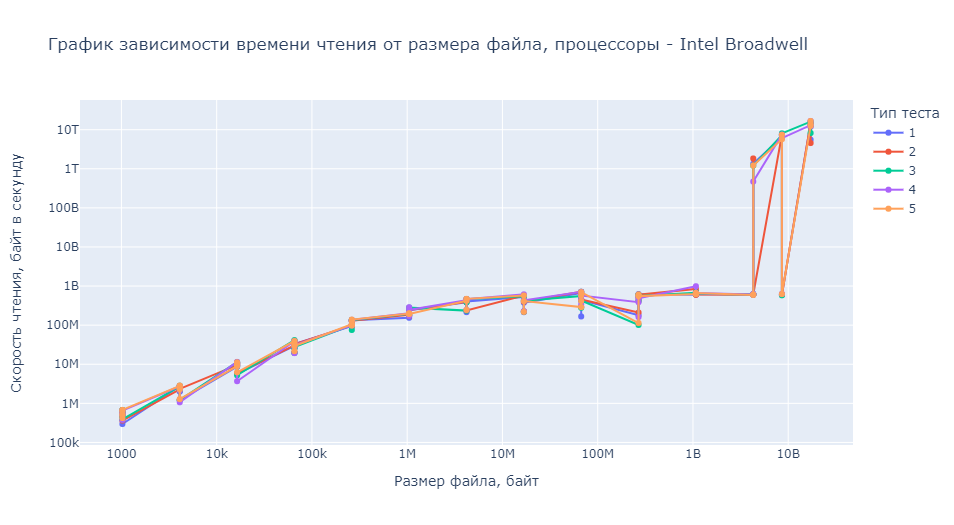
\includegraphics[height=9cm,keepaspectratio]{./test_graphs/read_broadwell.png}\\[0.1cm]
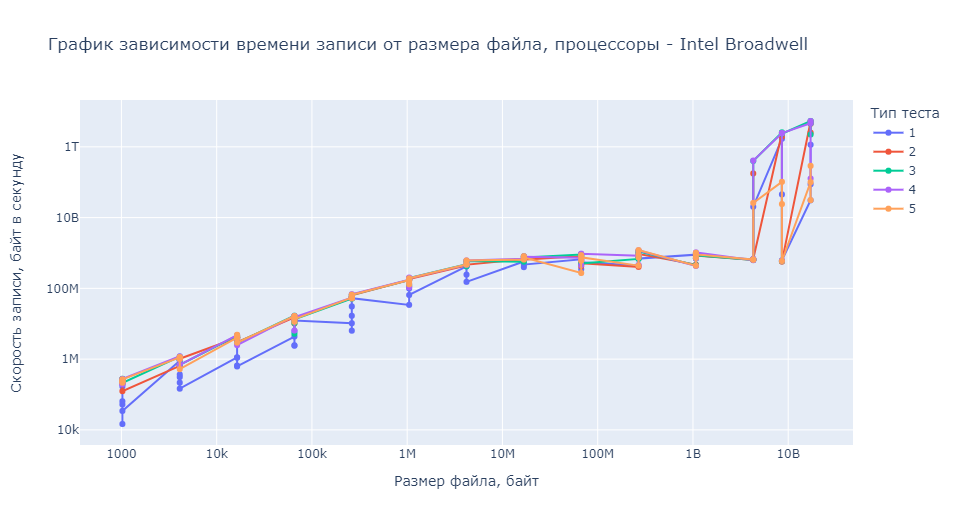
\includegraphics[height=9cm,keepaspectratio]{./test_graphs/write_broadwell.png}\\[0.1cm]
\caption{Тесты на разделе \textbf{Broadwell}}
\label{broadwell}
\end{figure}

\begin{figure}[h]
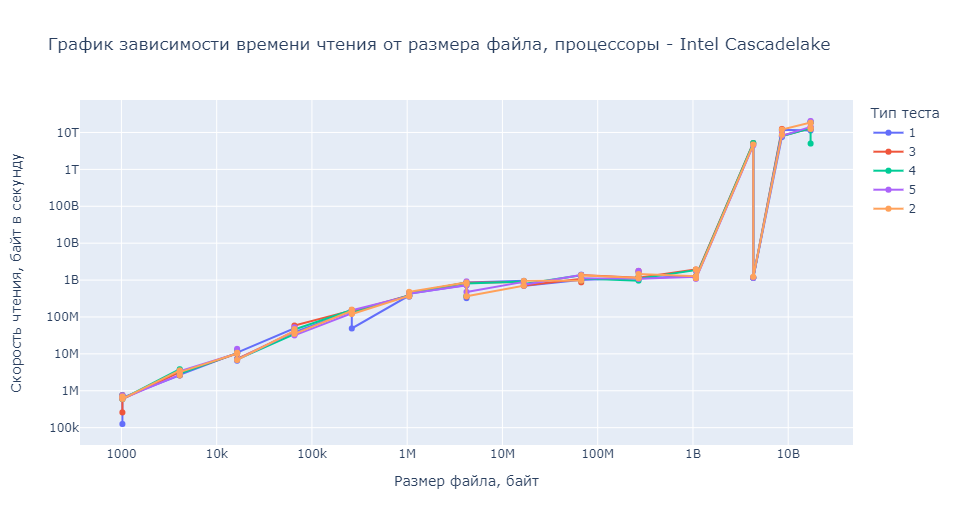
\includegraphics[height=9cm,keepaspectratio]{./test_graphs/read_cascadelake.png}\\[0.1cm]
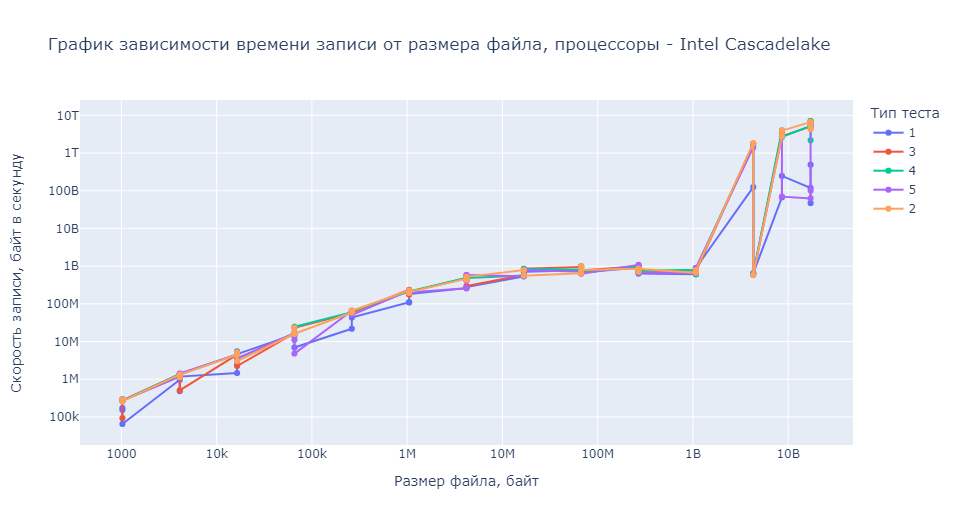
\includegraphics[height=9cm,keepaspectratio]{./test_graphs/write_cascadelake.png}\\[0.1cm]
\caption{Тесты на разделе \textbf{Cascade\_lake}}
\label{cascadelake}
\end{figure}

На графиках \ref{broadwell} можно увидеть зависимость скорости чтений и записи файлов. Замеры производительности были осуществлены на разделе кластера под названием \textbf{Broadwell}. Технические характеристики:
\begin{description}
    \item[$\bullet$] 136 вычислительных модулей на базе 16-ядерных процессоров Intel Xeon Broadwell
    \item[$\bullet$] Коммуникационная среда - Intel Omni-Path
    \item[$\bullet$] Каждый узел включает в себя 2 процессора Intel Xeon E5-2697Av4 и 128 Гб оперативной памяти
\end{description}


На графиках \ref{cascadelake} можно увидеть зависимость скорости чтений и записи файлов. Замеры производительности
были осуществлены на разделе кластера под названием \textbf{Cascade\_lake}. Технические характеристики:
\begin{description}
    \item[$\bullet$] 47 вычислительных модулей на базе 24-ядерных процессоров Intel Xeon Cascade Lake
    \item[$\bullet$] Коммуникационная среда - Intel Omni-Path
    \item[$\bullet$] Каждый узел включает в себя 2 процессора Intel Xeon Platinum 8268 2.90 GHz и 192 Гб
    оперативной памяти
\end{description}

Ввиду того, что на сервере присутствует дисковая квота в 17 гигабайт, запустить тест под номер 6 для сбора достаточной статистики оказалось невозможно, поэтому в данных присутствуют тесты с 1 по 5.

Если взглянуть на графики, то можно заметить, что для теста с одним размером файла было сделано несколько
запусков, при это скорость чтения-записи на этих тестах не отклоняется больше чем на 50\% от среднего
значения. Это значит, что lustre работает исправно и хорошо воспринимает параллельные потоки данных и
исправно функционирует, позволяя записывать данные параллельно.

Причём, как видно из графика, при увеличении размера файла, также растёт и скорость записи файла на диск,
это связано с тем, что растёт процент полезной нагрузки на сеть, ведь при записи или чтении файла MPI
сначала устанавливает связь со всеми процессами, они обмениваются между собой служебной информацией и
только после этого начинает переделывать сам файл для записи на диск. Также это можно связать с тем, что
файл начинает разбиваться на большее количество частей при записи на дисковое пространство. Этот процесс
называется File Striping - распределение одного файла между несколькими физическими или логическими
местами хранения файлов путём разбиения его на несколько частей. И как видно из графика, когда размер
файла достиг нескольких гигабайт распределение файла между несколькими серверами хранения стало более
агрессивное, что позволило ещё больше расспараллелить чтение-запись файла на диск, а как следствие
повысило скорость операций ввода-вывода.

 % Описание Экспериментальной части
\section{Заключение}
\label{sec:Chapter5} \index{Chapter5}

В ходе проведения обзора были выяснены основные подходы, которые применяются при тестировании 
файловых систем, а после применены при написании программы.  В ходе выполнения практической части
курсовой работы была разработана программа и набор тестов, который проводит нагрузочное тестирование
различных компонентов распределённой файловой системы lustre. Данную программу можно запустить как на одном узле,
так и  параллельно на всех узлах кластера и получить производительность всей системы на тестах, которые пользователь
укажет при запуске программы. Анализируя вывод программы, пользователь может понять какие части системы не
справляются с повышенной нагрузкой и перенастроить файловую систему для повышения производительности.
Данная программа была протестирована на Межведомственном суперкомпьюте МВС-10П, и показала, что данная
система очень хорошо справляются с нагрузками, которые реализованы в программе.


 % Заключение

\nocite{*}
\bibliographystyle{gost71u} % Для соответствия требованиям об оформлении списка литературы
\bibliography{references}

% \section*{Приложение}
\addcontentsline{toc}{section}{Приложение}
\label{sec:Apendix} \index{Apendix}

 

\end{document}
